\section{Introducción al Transistor Bipolar}

Un transistor de unión bipolar (BJT) es un dispositivo semiconductor que está compuesto por tres regiones dopadas, como se ilustra en la figura \ref{fig_ilustracion_bjt}. Existen dos tipos principales, \emph{npn} y \emph{pnp} según se haya dopado en cada región. Tal y como es representado, cada región tiene su propio nombre y no son intercambiables (cosa que se fundamentará más adelante).

\begin{figure}[!ht]
  \centering
    \begin{subfigure}[b]{0.7\textwidth}
    \centering
    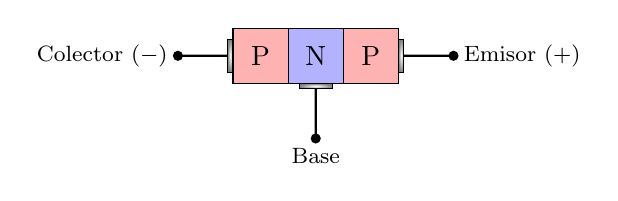
\begin{tikzpicture}[scale=0.7]
      \draw[fill=red!30] (0,0) rectangle node{P} (1,1);
      \draw[fill=blue!30] (1,0) rectangle node{N} (2,1);
      \draw[fill=red!30] (2,0) rectangle node{P} (3,1);
      \filldraw[thick] (-0.1,0.5) -- (-1,0.5) circle (2pt) node[left, font=\footnotesize] {Colector $(-)$};
      \filldraw[thick] (3.1,0.5) -- (4,0.5) circle (2pt) node[right, font=\footnotesize] {Emisor $(+)$};
      \filldraw[thick] (1.5,-0.1) -- (1.5,-1) circle (2pt) node[below, font=\footnotesize] {Base};
      \shadedraw[color=black,fill=gray,inner color=white,outer color=gray] (-0.1,0.2) rectangle (0,0.8);
      \shadedraw[color=black,fill=gray,inner color=white,outer color=gray] (3,0.2) rectangle (3.1,0.8);
      \shadedraw[color=black,fill=gray,inner color=white,outer color=gray] (1.2,-0.1) rectangle (1.8,0);
    \end{tikzpicture}
    \caption{Transistor PNP.}
  \end{subfigure}

  \vspace{5mm}

  \begin{subfigure}[b]{0.7\textwidth}
    \centering
    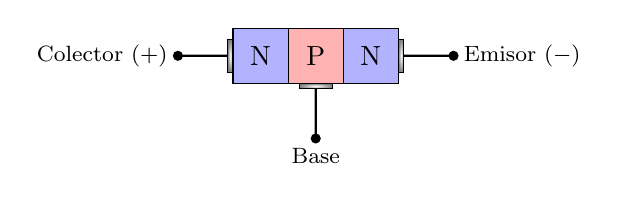
\begin{tikzpicture}[scale=0.7]
      \draw[fill=blue!30] (0,0) rectangle node{N} (1,1);
      \draw[fill=red!30] (1,0) rectangle node{P} (2,1);
      \draw[fill=blue!30] (2,0) rectangle node{N} (3,1);
      \filldraw[thick] (-0.1,0.5) -- (-1,0.5) circle (2pt) node[left, font=\footnotesize] {Colector $(+)$};
      \filldraw[thick] (3.1,0.5) -- (4,0.5) circle (2pt) node[right, font=\footnotesize] {Emisor $(-)$};
      \filldraw[thick] (1.5,-0.1) -- (1.5,-1) circle (2pt) node[below, font=\footnotesize] {Base};
      \shadedraw[color=black,fill=gray,inner color=white,outer color=gray] (-0.1,0.2) rectangle (0,0.8);
      \shadedraw[color=black,fill=gray,inner color=white,outer color=gray] (3,0.2) rectangle (3.1,0.8);
      \shadedraw[color=black,fill=gray,inner color=white,outer color=gray] (1.2,-0.1) rectangle (1.8,0);
    \end{tikzpicture}
    \caption{Transistor NPN.}
  \end{subfigure}
  \caption{Esquema ilustrativo de transistores BJT.}
  \label{fig_ilustracion_bjt}

  \caption{Esquema ilustrativo de transistores BJT.}
  \label{fig_ilustracion_bjt}
\end{figure}

Todas las ilustraciones, como la de la figura \ref{fig_ilustracion_bjt} presentan un defecto estético y didáctico. El hecho de dibujar las tres regiones de igual tamaño y sin distinción puede prestar a una confusión lógica y de compresión importante. En la realidad, como se explicó brevemente en el capítulo \ref{chpt_introduccion} el silicio debe ser dopado para formar material semiconductor tipo \emph{n} (usando Fósforo por ejemplo) y tipo \emph{p} (usando Boro por ejemplo). Pero en ningún caso se habló sobre cuánto Boro o cuanto Fósforo es suficiente o necesario para considerar dopado al semiconductor.

El motivo esencial de omitir la proporción de dopaje durante el estudio del diodo es debido a que no aporta mucho al análisis eléctrico. Sin embargo el diodo (como primera aproximación) es un poco más inofensivo en dicho aspecto, ya que no influye la proporción de dopaje y el tamaño de las regiones dopadas para comprender su funcionamiento. Sin embargo en el transistor la historia cambia un poco. Aquí, Carl, necesariamente deberá detallar cómo es la dimensión física de cada región y qué tan dopada está cada una, ya que esto es lo que hace que existan tres terminales denominadas ``emisor'', ``base'' y ``colector''.

\paragraph{La pregunta sobre los polos del transistor} Estudiando sobre semiconductores, Luis se encontró con estos dispositivos llamados transistores. Como había comprendido el funcionamiento del diodo pensó que el transistor sería casi análogo, pero le tomó un instante encontrar defectos en las explicaciones superficiales. Cuando Luis observó la representación de la figura \ref{fig_ilustracion_bjt} pensó ``¿Por qué no puedo intercambiar el emisor y el colector? ¿Qué hace que sean diferentes?''. 

\paragraph{El mito de los dos diodos y la barrera invisible} Usualmente, un transistor se explica utilizando una analogía que consiste en pensar el transistor como dos diodos en oposición. Si bien esto puede ``dar una idea'' sobre su comportamiento, no es una buena forma de adentrarse al tema. Vea lo que sucede cuando Luis dibuja en la pizarra el esquema mental: un transistor NPN conectado a una batería de \qty{12}{\volt} entre colector (positivo) y emisor (negativo) como muestra la figura \ref{fig_npn_no_polarizado}. Observe que el terminal positivo roba electrones del colector, dejando iones positivos cerca de la unión. 
\begin{figure}[!ht]
  \centering
  \begin{circuitikz}[scale=0.7]
  \draw[fill=blue!30] (0,0) rectangle node{N} (1,1);
  \draw[fill=red!30] (1,0) rectangle node{P} (2,1);
  \draw[fill=blue!30] (2,0) rectangle node{N} (3,1);
  \filldraw[thick] (-0.1,0.5) -- (-1,0.5) coordinate (E) node[below,font=\footnotesize]{E};
  \filldraw[thick] (3.1,0.5) -- (4,0.5) coordinate(C) node[below,font=\footnotesize]{C};
  \filldraw[thick] (1.5,-0.1) -- (1.5,-1) circle (2pt) node[below, font=\footnotesize] {B};
  \shadedraw[color=black,fill=gray,inner color=white,outer color=gray] (-0.1,0.2) rectangle (0,0.8);
  \shadedraw[color=black,fill=gray,inner color=white,outer color=gray] (3,0.2) rectangle (3.1,0.8);
  \shadedraw[color=black,fill=gray,inner color=white,outer color=gray] (1.2,-0.1) rectangle (1.8,0);
  \draw (E) to[short,*-] (-1,2) to[battery,invert,l={\(V_s=\qty{12}{\volt}\)}] (4,2) to[short,-*] (C);
\end{circuitikz}

  \caption{}
  \label{fig_npn_no_polarizado}
\end{figure}

``Si el colector es tipo N y está a \qty{12}{\volt}, sus electrones libres son arrastrados por el positivo de la batería'', razona Luis, intentando unir los conceptos. ``Por el otro lado, el emisor también es N, así que el negativo de la batería empuja sus electrones hacia la base tipo P. Pero la base está llena de huecos... que son, viéndolo así, espacios vacíos. Si esta base está desconectada, los electrones del emisor que llegan ahí se quedan estancados, sin un circuito por donde escapar. Entonces, la zona P actúa simplemente como un aislante pasivo que separa dos regiones con carga... ¿¡Todo este componente no es más que un solo capacitor complicado!?''.

Carl sonríe y niega lentamente con la cabeza. ``Es un razonamiento perfectamente lógico si estuviéramos conectando componentes discretos, pero ahí radica la trampa. Estás imaginando el material tipo P como un simple dieléctrico y tratando a las regiones N como placas de metal. Pensarlo como un capacitor, o incluso como dos diodos soldados por sus ánodos, es un callejón sin salida. En la realidad, el secreto para que los electrones atraviesen esa barrera reside en un delicado equilibrio de dopaje y en un diseño físico extremo''.

\paragraph{Las dos zonas de deplexión}
Carl toma una tiza y dibuja el interior del transistor. Le señala a Luis que, al haber tres bloques, existen \emph{dos} zonas de deplexión: la unión Base-Emisor y la unión Base-Colector, como se representa en la figura \ref{fig_zona_de_deplexión}. 

\begin{figure}[!ht]
  \centering
  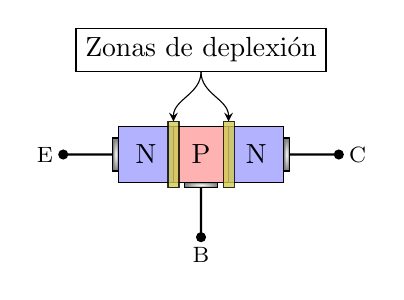
\begin{tikzpicture}[scale=0.7,>=stealth]
  \draw[fill=blue!30] (0,0) rectangle node{N} (1,1);
  \draw[fill=red!30] (1,0) rectangle node{P} (2,1);
  \draw[fill=blue!30] (2,0) rectangle node{N} (3,1);
  \filldraw[thick] (-0.1,0.5) -- (-1,0.5) circle (2pt) node[left, font=\footnotesize] {E};
  \filldraw[thick] (3.1,0.5) -- (4,0.5) circle (2pt) node[right, font=\footnotesize] {C};
  \filldraw[thick] (1.5,-0.1) -- (1.5,-1) circle (2pt) node[below, font=\footnotesize] {B};
  \shadedraw[color=black,fill=gray,inner color=white,outer color=gray] (-0.1,0.2) rectangle (0,0.8);
  \shadedraw[color=black,fill=gray,inner color=white,outer color=gray] (3,0.2) rectangle (3.1,0.8);
  \shadedraw[color=black,fill=gray,inner color=white,outer color=gray] (1.2,-0.1) rectangle (1.8,0);
  \draw[fill=yellow!60!gray,opacity=0.8] (0.9,-0.1) rectangle ++(.2,1.2);
  \draw[fill=yellow!60!gray,opacity=0.8] (1.9,-0.1) rectangle ++(.2,1.2);
  \node[draw, above] (T) at (1.5,2) {Zonas de deplexión};
  \draw[->] (T.south) to[out=270,in=90] (1,1.1);
  \draw[->] (T.south) to[out=270,in=90] (2,1.1);
\end{tikzpicture}

  \caption{Zonas de deplexión en un transistor.}
  \label{fig_zona_de_deplexión}
\end{figure}

Con los \qty{12}{\volt} en el colector y el emisor a tierra (y la base desconectada como se representó en la figura \ref{fig_npn_no_polarizado}), la unión Base-Colector y la unión Base-Emisor sufren un pequeño desplazamiento de cargas.

\paragraph{La trampa de la neutralidad y la base flotante} Carl le transmite un gesto de tranquilidad a Luis. ``Es normal que resulte confuso, pero recuerda siempre los fundamentos que vimos en los diodos: los materiales tipo \emph{p} y tipo \emph{n} son, en su origen, eléctricamente neutros. Esto se debe a que, aunque tengan huecos o electrones libres, el átomo dopante que aporta ese electrón o hueco extra también tiene un protón correspondiente en su núcleo. Todo está balanceado. Solo cuando los electrones se desplazan —por ejemplo, al conectar una batería— es que dejas atrás iones fijos positivos o negativos''. A lo que Luis responde: ``¿Pero y qué sucede con la base desconectada?''.

``Como tienes una zona de deplexión en las interfaces de las zonas \emph{n} y \emph{p}, se crea un campo eléctrico interno que se opone al flujo de electrones'', explica Carl. ``Pero tu batería de \qty{12}{\volt} aplica una gran diferencia de potencial sobre todo el conjunto. La unión Base-Colector absorbe casi todo el impacto y se ensancha, mientras que la Base-Emisor apenas se altera. Esto provoca que la base adquiera un potencial flotante, un poco mayor al polo negativo de la batería. Es decir, su potencial no es cero''. 

Carl hace una pausa y, respondiendo a la duda del equivalente que planteó Luis anteriormente, concluye: ``Así que, complementando tu idea, un transistor con la base desconectada no sería un solo capacitor... más bien se comporta como \emph{dos} capacitores conectados en serie. ¿Súper loco, verdad?''.

\paragraph{Conexión de la base}
``¿Qué pasa si ahora le aplicamos \qty{0.7}{\volt} a la base respecto al emisor?'', pregunta Carl. 

Piense un segundo sobre esta pregunta. Si observa el esquema de la figura \ref{fig_npn_no_polarizado} y añade una fuente de \qty{0.7}{\volt} en la base, ¿qué camino seguirán las cargas? La unión Base-Emisor se comporta como un diodo convencional, por lo que es seguro afirmar que fluirán cargas desde el emisor hacia la base. Pero, ¿qué sucede con el colector?

\paragraph{El diseño físico de un transistor} Carl explica que, si el transistor fuera perfectamente simétrico, la corriente simplemente fluiría hacia la base o se repartiría sin un propósito claro. Sin embargo, en la realidad un transistor no se comporta de esta manera; su principal característica es que la corriente que sale por el terminal de la base es ínfima comparada con la que llega al colector. ``¿Por qué ocurre esto?'', interrumpe Luis, intrigado.

Esto se debe a que el transistor no es un par de diodos ni tampoco un bloque \emph{NPN} simétrico. Su diseño físico real, representado en la figura \ref{fig_npn_representacion_real}, revela proporciones y niveles de dopaje muy específicos. Observe que no solo los tamaños del emisor, base y colector son diferentes, sino que la densidad de portadores también cambia en cada región. El emisor está fuertemente dopado (es decir, es un material con una enorme cantidad de electrones libres agregados). El colector, aunque es la región de mayor tamaño para disipar el calor, tiene un dopaje moderado. Finalmente, la base es físicamente la región más estrecha y está dopada de forma muy débil. Esta asimetría es la clave para que los electrones del emisor saturen la base y, en su gran mayoría, terminen saltando hacia el colector.

\begin{figure}[!ht]
  \centering
  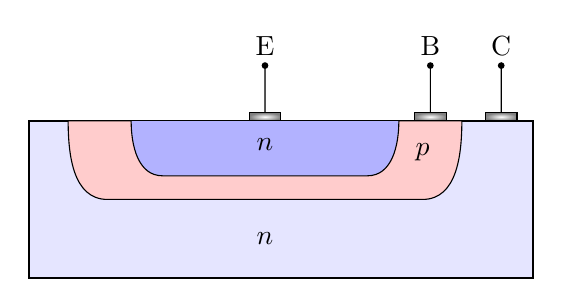
\begin{tikzpicture}
  \draw[fill] (2.1,1) -- ++(0,0.7) circle (1pt) node[above]{B};
  \draw[fill] (0,1) -- ++(0,0.7) circle (1pt) node[above]{E};
  \draw[fill] (3,1) -- ++(0,0.7) circle (1pt) node[above]{C};
  \shadedraw[color=black,fill=gray,inner color=white,outer color=gray] (1.9,1) rectangle (2.3,1.1);
  \shadedraw[color=black,fill=gray,inner color=white,outer color=gray] (-.2,1) rectangle (.2,1.1);
  \shadedraw[color=black,fill=gray,inner color=white,outer color=gray] (2.8,1) rectangle (3.2,1.1);
  \draw[fill=blue!10,thick] (-3,-1) rectangle (3.4,1);
  \draw[fill=blue!30] (-2,0.2) rectangle (2,1);
  \draw[fill=red!20] (-2.5,1) to[out=270,in=180]
    (-2,0) -- (2,0) to[out=0,in=270]
    (2.5,1) -- (1.7,1) to[out=270,in=0]
    (1.3,0.3) -- (-1.3,0.3) to[out=180,in=270] 
    (-1.7,1) -- cycle;
  \node at (0,-.5) {\(n\)};
  \node at (0,.7) {\(n\)};
  \node at (2,.6) {\(p\)};
\end{tikzpicture}

  \caption{Esquema realista del diseño físico y proporciones de un transistor.}
  \label{fig_npn_representacion_real}
\end{figure}

Volviendo al concepto de la barrera de \qty{0.7}{\volt}, Luis analiza la situación: ``Entonces, al superar la barrera de potencial del silicio, la unión Base-Emisor se polariza en directa. Su zona de deplexión se reduce dramáticamente y el emisor, que está fuertemente dopado, inyecta una cantidad masiva de electrones libres hacia la base''.

``¡Exacto! Y aquí es donde el diseño físico rompe las reglas convencionales'', asiente Carl con una sonrisa. ``La base tiene huecos, sí, pero el fabricante la hace \emph{extremadamente delgada} (apenas unos micrómetros) y la dopa \emph{muy débilmente}. Cuando esa avalancha de electrones ingresa a la base, hay tan pocos huecos disponibles que solo alrededor del 1\% de los electrones logra chocar, recombinarse y salir por el cable de la base''.

Carl dibuja flechas gruesas cruzando la región central. ``El 99\% restante de los electrones entra con tanta energía cinética que atraviesa la minúscula base sin encontrar un solo hueco para recombinarse. Antes de que pierdan impulso, se asoman al abismo: la enorme zona de deplexión de la unión Base-Colector''.

Luis, visualizando el panorama completo, concluye: ``Claro... Esa unión estaba en inversa para bloquear a los huecos de la base, pero para los electrones libres que vienen lanzados desde el emisor, ¡ese campo eléctrico actúa como un acelerador directo hacia el colector!''.

``¡Precisamente!'', exclama Carl. ``Esa tensión de \qty{12}{\volt} mantiene un campo eléctrico muy intenso en la zona de deplexión del colector. Cuando los electrones sobreviven al cruce de la base y tocan el borde de esa región, el campo eléctrico los captura y los arrastra con gran fuerza hacia el terminal positivo de la batería, conformando la corriente principal del circuito''.

\paragraph{Visualización real de un BJT} Para finalizar la idea de introducción al transistor, observe el transistor fotografiado bajo un microscópio en la figura \ref{fig_bjt_under_microscope} capturada por \cite{article_transistors}.

\begin{figure}[!ht]
  \centering
  \includegraphics[height=8cm]{chapters/01_capitulo/media/bin/bjt_under_microscope.png}
  \caption{Transistor de unión bipolar capturado bajo el microscópio electrónico.}
  \label{fig_bjt_under_microscope}
\end{figure}

La figura \ref{fig_bjt_under_microscope} demuestra el formato físico de un transistor BJT. Para poder comprender la imagen se dará una breve explicación de qué se está visualizando. Las micrografías obtenidas por Microscopía Electrónica de Barrido (MEB) (imágenes capturadas con un microscópio electrónico) revelan la naturaleza tridimensional del transistor, caracterizada por tres escalones verticales bien definidos. Estos desniveles geométricos corresponden a surcos de aislamiento (\textit{trench isolation}) grabados a diferentes profundidades críticas en la oblea de silicio: el aislamiento del emisor ($\ge 0.5\,\mu\text{m}$), el de la base ($\ge 1.5\,\mu\text{m}$) y el del colector ($\ge 1.0\,\mu\text{m}$). La implementación de estas barreras físicas, posteriormente rellenadas con material dieléctrico, es fundamental en la arquitectura microelectrónica para confinar portadores y prevenir interferencias eléctricas o cortocircuitos entre los terminales de transistores adyacentes que coexisten en el mismo sustrato. 

La inclusión de la figura \ref{fig_bjt_under_microscope} es para que observe que físicamente las regiones de emisor, colector y base son de diferentes tamaños y tienen diferentes propósitos, como ya se explicó anteriormente.

\paragraph{¿El colector como emisor?} Para dar una respuesta concluyente a la pregunta inicial: tras analizar el diseño interno, resulta evidente que el transistor es físicamente asimétrico. Cada región tiene un dopaje y un volumen específicos, por lo que emisor y colector no son intercambiables. Sin embargo, ¿qué sucede si conectamos el componente al revés, invirtiendo estos dos terminales? Técnicamente, el dispositivo operará en lo que se conoce como \emph{región activa inversa}. El transistor funcionará, pero de manera sumamente ineficiente. Al obligar al gran colector (débilmente dopado) a emitir electrones y al minúsculo emisor a intentar recolectarlos, la ganancia de corriente se desploma. Peor aún, la unión Base-Emisor no está diseñada para soportar altas tensiones en inversa, por lo que el componente podría dañarse. En resumen, conectarlo al revés es desperdiciar por completo la genialidad y precisión de su diseño físico.

